\section{Αποτελέσματα εκπαίδευσης}
Σε αυτό το σημείο, παρουσιάζονται τα διαγράμματα που δείχνουν την πορεία εξέλιξης της τιμής των αντικειμενικών συναρτήσεων που χρησιμοποιούνται κατά την εκπαίδευση, οι οποίες είναι όπως έχει αναφερθεί το MSE, RMSE και MAE, για τα δύο διαφορετικά μοντέλα που εκπαιδεύτηκαν, το fully connected, και το convolutional.

\subsection{Πλήρως διασυνδεδεμένη αρχιτεκτονική}

Κατά την διαδικασία της εκπαίδευσης, κάθε νευρώνας εκτελεί ένα σταθμισμένο άθροισμα, το οποίο τελικά δίνεται ως είσοδος στη συνάρτηση ενεργοποίησης, ώστε να παραχθεί η έξοδος του νευρώνα. Οι πράξεις αυτές εκτελούνται γρήγορα σε σχέση με τις πράξεις που είναι απαραίτητες στις άλλες αρχιτεκτονικές, (CNN, CRNN κλπ). Στα διαγράμματα \ref{fig:FC_MSE}, \ref{fig:FC_RMSE} και \ref{fig:FC_MAE}, φαίνονται με τη σειρά η εξέλιξη των τιμών του MSE, RMSE και MAE αντίστοιχα. Τα test data χρησιμοποιούνται κατά το πέρας της εκπαίδευσης, για την τελική αξιολόγηση του μοντέλου και παρουσιάζονται σε επόμενη υποενότητα. Τα διαγράμματα αυτά περιγράφουν ουσιαστικά την \textit{ιστορία} του μοντέλου.

Το μοντέλο, ξεκινά με τελείως τυχαίες προβλέψεις, που αιτιολογούν και το εξαιρετικά μεγάλο σφάλμα κατά την αρχή της εκπαίδευσης, ενώ στη συνέχεια, \textit{μαθαίνει}, να βγάζει συμπεράσματα από τα χαρακτηριστικά των διανυσμάτων εισόδου. Με τον όρο \textit{epoch} στον άξονα \textit{Χ}, υποδηλώνεται ένα \textbf{πλήρες} πέρασμα του dataset από τον αλγόριθμο. Το μοντέλο ξεκινά να συγκλίνει περίπου μετά από 350 εποχές, όπως φαίνεται από τη συνάρτηση απώλειας MSE, όπου το σφάλμα παραμένει σχετικά σταθερό. Σε εκείνο το σημείο αξιοποιείται η τεχνική Early Stopping, όπου όταν το σφάλμα δεν μειώνεται για έναν προκαθορισμένο αριθμό εποχών, τότε τερματίζεται η διαδικασία της εκπαίδευσης για την αποφυγή σπατάλης υπολογιστικών πόρων και προφανώς, χρόνου. 

Γίνεται επίσης εμφανές, το γεγονός ότι οι καμπύλες που δείχνουν την απόδοση στα training και στα validation data απέχουν κάποια απόσταση μεταξύ τους. Αυτό είναι αναμενόμενο, και ο λόγος που η καμπύλη που αφορά τα δεδομένα εκπαίδευσης είναι πάντα κάτω από την καμπύλη του validation, είναι το γεγονός ότι τα νευρωνικά δίκτυα, και ιδιαίτερα οι fully connected αρχιτεκτονικές, έχουν την τάση να 'απομνημονεύουν' τα δεδομένα εισόδου, με αποτέλεσμα να έχουν χειρότερη απόδοση σε δεδομένα που 'βλέπουν' πρώτη φορά. Η περίπτωση στην οποία η απόσταση μεταξύ των δύο καμπυλών μεγαλώνει όσο περνάνε οι εποχές λέγεται \textbf{\textit{overfitting}} και τα επίπεδα Dropout, έχουν χρησιμοποιηθεί για την αντιμετώπισή του.

\begin{figure}[h!]
  \centering
  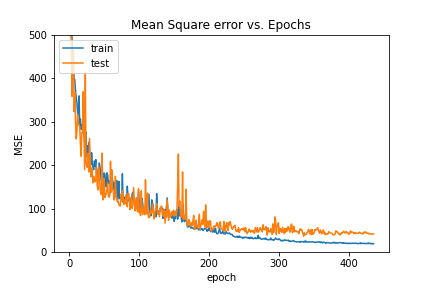
\includegraphics[width=\textwidth]{images/FC_MSE.png}
  \caption{Ιστορικό τιμών του MSE για την Fully Connected αρχιτεκτονική.}
  \label{fig:FC_MSE}
\end{figure}

\begin{figure}[h!]
  \centering
  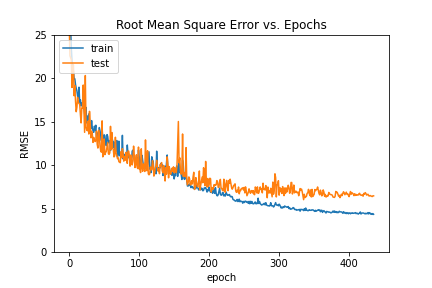
\includegraphics[width=\textwidth]{images/FC_RMSE.png}
  \caption{Ιστορικό τιμών του RMSE για την Fully Connected αρχιτεκτονική.}
  \label{fig:FC_RMSE}
\end{figure}

\begin{figure}[h!]
  \centering
  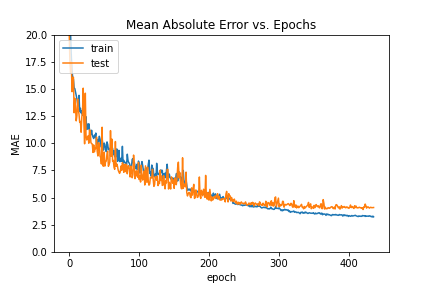
\includegraphics[width=\textwidth]{images/FC_MAE.png}
  \caption{Ιστορικό τιμών του MAE για την Fully Connected αρχιτεκτονική.}
  \label{fig:FC_MAE}
\end{figure}

\newpage
\subsection{Συνελικτική αρχιτεκτονική}

Τα αντίστοιχα αποτελέσματα για την convolutional δομή, παρουσιάζονται σε αυτή την υποενότητα, στα Σχήματα \ref{fig:CNN_MSE}, \ref{fig:CNN_RMSE} και \ref{fig:CNN_MAE} για τα MSE, RMSE και MAE αντίστοιχα. Αξίζει να σημειωθεί το γεγονός, πως το CNN, χρειάζεται τις μισές περίπου εποχές για να φτάσει στο τοπικό ελάχιστο της συνάρτησης, χωρίς αυτό να σημαίνει όμως ότι συγκλίνει γρηγορότερα από άποψη χρόνου. Η πράξη της συνέλιξης είναι ιδιαίτερα αργή από υπολογιστική άποψη, και αυτός είναι ο κυριότερος λόγος για αυτό. Παρατηρείται επίσης, πως οι καμπύλες έχουν μεγαλύτερη κλίση στην αρχή της εκπαίδευσης. 

Τα CNN είναι πιο εύρωστα στο φαινόμενο του overfitting, οπότε δεν χρειάστηκε να προστεθούν επίπεδα Dropout για την εκπαίδευση του μοντέλου. Το CNN κάνει λάθος περίπου $3.5^o$, στην πρόβλεψη της γωνίας άφιξης, δηλαδή είναι περίπου 50\% καλύτερο από την fully connected αρχιτεκτονική που έχει μέσο σφάλμα σχεδόν $6.5^o$.

\begin{figure}[h!]
  \centering
  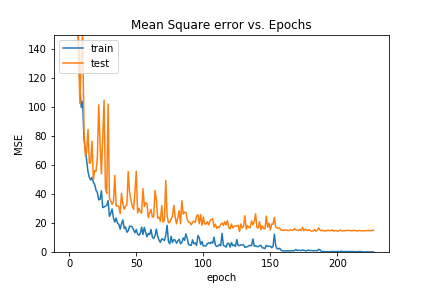
\includegraphics[width=\textwidth]{images/CNN_MSE.png}
  \caption{Ιστορικό τιμών του MSE για την συνελικτική αρχιτεκτονική.}
  \label{fig:CNN_MSE}
\end{figure}

\begin{figure}[h!]
  \centering
  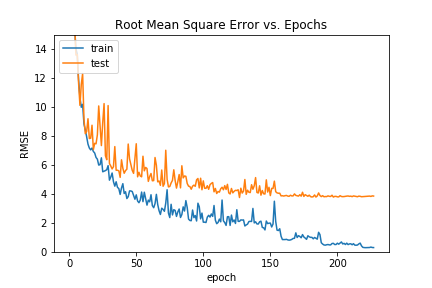
\includegraphics[width=\textwidth]{images/CNN_RMSE.png}
  \caption{Ιστορικό τιμών του RMSE για την συνελικτική αρχιτεκτονική.}
  \label{fig:CNN_RMSE}
\end{figure}

\begin{figure}[h!]
  \centering
  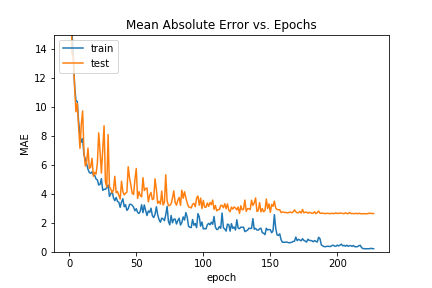
\includegraphics[width=\textwidth]{images/CNN_MAE.png}
  \caption{Ιστορικό τιμών του MAE για την Fully Connected αρχιτεκτονική.}
  \label{fig:CNN_MAE}
\end{figure}


\subsection{Χρόνοι σύγκλισης}
Εδώ παρουσιάζονται με συνοπτικό τρόπο οι χρόνοι σύγκλισης των δύο μοντέλων στον Πίνακα \ref{tab:model_times}. Σημειώνεται πως ο χρόνος που χρειάζονται και τα δύο μοντέλα για να συγκλίνουν είναι σημαντικά μικρότερος από άλλα μοντέλα που έχουν κατασκευαστεί με παρόμοιο στόχο.

\begin{table}[h!]
    \centering
    \begin{tabularx}{0.8\textwidth} { 
  | >{\centering\arraybackslash}X 
  | >{\centering\arraybackslash}X 
  | >{\centering\arraybackslash}X | }
     \hline
     Model & Epochs & Time (mins) \\[5pt]
     \hline
     Fully Connected & 436 & 125.36 \\[5pt]
    \hline
    Convolutional & 228 & 183.36 \\[5pt]
    \hline
    \end{tabularx}
    \caption{Σύγκριση χρόνων σύκλισης των μοντέλων σε εποχές και λεπτά.}
    \label{tab:model_times}
\end{table}{}

\section{Αποτελέσματα εκτίμησης}

Η απόδοση των μοντέλων αξιολογήθηκε ως προς την ικανότητά τους να εκτιμήσουν την DOA, σε δεδομένα που αντιμετωπίζουν πρώτη φορά. Αυτή ακριβώς είναι η αξία του διαχωρισμού σε train-validation-test δεδομένα, δηλαδή το ότι παρέχεται μια εγγύηση ως προς την αξιοπιστία των δεδομένων. Εκτός από τις συναρτήσεις που έχουν ήδη αναφερθεί (MSE, RMSE, MAE), χρησιμοποιούνται σε αυτό το στάδιο το \textit{Accuracy} ως προς την ταξινόμηση, των μοντέλων σε τρεις κατηγορίες προβλέψεων. Μια DOA θεωρείται σωστά ταξινομημένη εφόσον η διαφορά της προβλεπόμενης γωνίας άφιξης από την πραγματική είναι μικρότερη ή ίση με 5, 10 και 15 μοίρες για τις μετρικές Acc5, Acc10 και Acc15 αντίστοιχα. Για κάθε περιθώριο σφάλματος, το classification accuracy υπολογίζεται όπως φαίνεται στην εξίσωση \ref{eq:DOA_Accuracy}.

\begin{CEquation}
\begin{split}
    Accuracy(\%) = \frac{100}{n}\sum_{i=1}^nd_i\\
    \text{όπου } d_i = 
        \begin{cases}
         1 & \text{αν}\;|y_i-\hat{y_i}|<err\\
         0 & \text{αλλού}
         \end{cases} 
\end{split}
\label{eq:DOA_Accuracy}
\end{CEquation}

Τα αποτελέσματα των μοντέλων κατά το testing, φαίνονται στον πίνακα \ref{tab:model_accuracies}. Σημειώνεται πως τα 'Test Noise Signals' (TNS στον πίνακα) είναι τα burst θορύβου που δημιουργήθηκαν για τους σκοπούς αυτής της εργασίας. Στην περίπτωση του CNN, δοκιμάστηκε η απόδοσή του στην εκτίμηση της γωνίας άφιξης, όταν το σήμα εισόδου είναι κάτι τελείως διαφορετικό από αυτά που έχει δει στην εκπαίδευση, όπως φωνή ή μουσική. Το CNN φαίνεται πως γενικεύει εξαιρετικά σε νέα δεδομένα, επιτυγχάνοντας ένα ελάχιστο classification accuracy 79\%, και μέγιστο  85\%. 

\begin{table}[h!]
    \centering
    \begin{tabularx}{\textwidth} { 
  | >{\centering\arraybackslash}X 
  | >{\centering\arraybackslash}X 
  | >{\centering\arraybackslash}X
  | >{\centering\arraybackslash}X
  | >{\centering\arraybackslash}X
  | >{\centering\arraybackslash}X
  | >{\centering\arraybackslash}X | }
     \hline
     Dataset & MSE & RMSE & MAE & Acc5(\%) & Acc10(\%) & Acc15(\%)\\[5pt]
     \hline
     \multicolumn{7}{|c|}{Fully Connected Architecture} \\[5pt]
     \hline
     TNS & 40.5 & 6.4 & 4 & 89 & 97 & 98 \\[5pt]
     \hline
     \multicolumn{7}{|c|}{Convolutional Architecture} \\[5pt]
     \hline
     TNS & 11.3 & 3.4 & 2.3 & 96 & 99 & 100 \\[5pt]
     \hline
     Voice & 82.8 & 9.1 & 7.0 & 79 & 89 & 95 \\[5pt]
     \hline
     Bongo & 212.4 & 14.6 & 10.5 & 80 & 90 & 96 \\[5pt]
     \hline
     Cello & 123.0 & 11.1 & 9.1 & 88 & 95 & 98 \\[5pt]
     \hline
     Guitar & 130.7 & 11.4 & 9.3 & 87 & 94 & 97 \\[5pt]
     \hline
     Xyloph. & 212.4 & 14.6 & 10.5 & 80 & 90 & 96 \\[5pt]
     \hline
     CNN Mean & 128.8 & 10.7 & 8.1 & 85 & 93 & 97 \\[5pt]
     \hline
     
    \end{tabularx}
    \caption{Αποτελέσματα εκτίμισης γωνίας άφιξης για διαφορετικά σήματα διέγερσης.}
    \label{tab:model_accuracies}
\end{table}{}

Είναι εμφανές πως το CNN, έχει μακράν καλύτερα αποτελέσματα από το αντίστοιχο Fully Connected μοντέλο και για αυτόν τον λόγο κρίθηκε πως είχε νόημα να δοκιμαστεί η απόδοσή του σε διαφορετικές συνθήκες. Σημειώνεται πως οι BRIR που χρησιμοποιούνται σε αυτή την εργασία προκύπτουν από πραγματικά δωμάτια, ενώ στα περισσότερα άλλα συστήματα εντοπισμού γωνίας άφιξης, χρησιμοποιούνται συνήθως simulated δωμάτια.

\section{Σύγκριση με άλλες μεθόδους}
Η υποενότητα αυτή επικεντρώνεται στη σύγκριση της προτεινόμενης μεθόδου με άλλες δημοσιευμένες μεθόδους εκτίμησης DOA που χρησιμοποιούν τεχνικές μηχανικής μάθησης. Για το μοντέλο αυτής της εργασίας χρησιμοποιούνται οι μέσες τιμές κάθε μετρικής που προκύπτουν από εκτιμήσεις του CNN, όπως φαίνονται στον πίνακα \ref{tab:model_accuracies}, ενώ στα άλλα μοντέλα χρησιμοποιούνται τα καλύτερα αποτελέσματα που έχουν επιτευχθεί. Τονίζεται πως δεν χρησιμοποιούνται παντού οι ίδιες μετρικές, οπότε αναφέρονται όσες είναι διαθέσιμες. Σε αντίθετη περίπτωση χρησιμοποιούνται best και worst case αποτελέσματα στη θέση των Acc5 και Acc15 αντίστοιχα. Στον πίνακα \ref{tab:model_comparisons1} παρουσιάζονται οι συγκρίσεις μεταξύ των μοντέλων.

\begin{table}[h!]
    \centering
    \begin{tabularx}{\textwidth} { 
  | >{\centering\arraybackslash}X 
  | >{\centering\arraybackslash}X 
  | >{\centering\arraybackslash}X 
  | >{\centering\arraybackslash}X | }
     \hline
     Model & Acc5(\%) & Acc10(\%) & Acc15(\%) \\[5pt]
     \hline
    Proposed Model & 85 & 93 & 97 \\[5pt]
    \hline
    Intensity-CRNN (Simulated RIR) \cite{Perotin2019} & 54.3 & 94.4 & 98.9\\[5pt]
    \hline
    Intensity-CRNN (Real RIR) \cite{Perotin2019}& 26.2 & 62.6 & 78.1 \\[5pt]
    \hline
    DoaNet \cite{Perotin2019}& 59.3 & - & 95.4 \\[5pt]
    \hline
    CNN+masking \cite{Zhang2019}& 65.8 & - & 87.0 \\[5pt]
    \hline
    \end{tabularx}
    \caption{Σύγκριση DOA Accuracy της προτεινόμενης μεθόδου, με άλλες δημοσιευμένες μεθόδου.}
    \label{tab:model_comparisons1}
\end{table}{}

Για τις μεθόδους που συγκρίθηκαν στον πίνακα \ref{tab:model_comparisons1}, οι πίνακες \ref{tab:model_comparisons2} και \ref{tab:model_comparisons3} παρουσιάζουν τις διαφορετικές αρχιτεκτονικές νευρωνικών δικτύων και τα datasets που χρησιμοποιήθηκαν για την εκπαίδευσή τους. Ελέγχοντας τους δύο πίνακες ταυτόχρονα, παρατηρείται ότι η προτεινόμενη μέθοδος εξαρτάται από δεδομένα που προέρχονται από πραγματικά δωμάτια, και σε συνδυασμό με την μέθοδο \textit{profiling} που κατασκευάστηκε και αναλύθηκε στο κεφάλαιο \ref{sec:data_compression}, επιτυγχάνει εξαιρετικά αποτελέσματα ακόμα και με σχετικά μικρό dataset εκπαίδευσης. Ακόμα ένα πλεονέκτημα της προτεινόμενης μεθόδου είναι η αξιοσημείωτη ταχύτητα σύγκλισης, ολοκληρώνοντας της διαδικασία της εκπαίδευσης σε 3.5 ώρες (για το μοντέλο CNN το οποίο απαιτεί και τον περισσότερο χρόνο).

\begin{table}[h!]
    \centering
    \begin{tabularx}{\textwidth} { 
  | >{\centering\arraybackslash}X 
  | >{\centering\arraybackslash}X 
  | >{\centering\arraybackslash}X 
  | >{\centering\arraybackslash}X | }
     \hline
     Model & Architecture & R/C & NN Inputs \\[5pt]
     \hline
    Proposed Model & 1D-CNN & R & ILD+ITD Profiles \\[5pt]
    \hline
    Intensity-CRNN & 2D-CRNN & C & Acoustic Intensity Vectors\\[5pt]
    \hline
    DoaNet & 2D-CRNN & C & Magnitude + Phase Spectrograms \\[5pt]
    \hline
    CNN+masking & CRNN & C & Magnitude Spectrograms \\[5pt]
    \hline
    \end{tabularx}
    \caption{Σύγκριση των μοντέλων ως προς την αρχιτεκτονική που χρησιμοποιήθηκε και τις εισόδους. Με R/C σημειώνεται αν το νευρωνικό ήταν τύπου regression ή classification.}
    \label{tab:model_comparisons2}
\end{table}{}

\begin{table}[h!]
    \centering
    \begin{tabularx}{\textwidth} { 
  | >{\centering\arraybackslash}X 
  | >{\centering\arraybackslash}X 
  | >{\centering\arraybackslash}X 
  | >{\centering\arraybackslash}X | }
     \hline
     Model & Signals & Real Rooms & Training Vectors \\[5pt]
     \hline
    Proposed Model & Noise Burst & Yes & 6334 \\[5pt]
    \hline
    Intensity-CRNN & Bref Corpus & No & 127800 \\[5pt]
    \hline
    DoaNet & Real-life sound events & No & - \\[5pt]
    \hline
    CNN+masking & TIMIT+ChiME3 & No & 24000 \\[5pt]
    \hline
    \end{tabularx}
    \caption{Σύγκριση των μοντέλων ως προς τα δεδομένα που χρησιμοποιήθηκαν για την εκπαίδευσή τους.}
    \label{tab:model_comparisons3}
\end{table}{}

\newpage
\section{Σύγκριση αποτελεσμάτων με και χωρίς συμπίεση}

Για την επιβεβαίωση της καλής λειτουργίας του αλγορίθμου συμπίεσης, συγκρίθηκαν τα αποτελέσματα με και χωρίς τη χρήση του. Εκπαιδεύτηκαν δηλαδή μοντέλα εκ νέου, χωρίς να συμπιεστούν τα δεδομένα. Χρησιμοποιώντας στη συνέχεια τις ίδιες αρχιτεκτονικές τα μοντέλα εκπαιδεύτηκαν με τα συμπιεσμένα δεδομένα. Παρατίθενται τα αποτελέσματα του παραπάνω πειράματος, το οποίο εκτελέστηκε για fully connected και για convolutional δομές στους Πίνακες \ref{tab:model_comparisons4} και \ref{tab:model_comparisons5}.

\begin{table}[h!]
    \centering
    \begin{tabular}{|c|c|c|c|c|c|}
     \hline
     \multicolumn{6}{|c|}{Fully Connected architecture} \\[5pt]
     \hline
      & MSE & MAE & Acc5(\%) & Acc10(\%) & Time(min) \\[5pt]
     \hline
    \textbf{{\small Compressed}} & 19.9 & 3.4 & 89 & 99 & 10.93 \\[5pt]
    \hline
    {\small Uncompressed} & 49.2 & 5.3 & 83 & 96 & 41.78 \\[5pt]
    \hline
    \end{tabular}
    \caption{Σύγκριση accuracy και χρόνων στις fully connected αρχιτεκτονικές για συμπιεσμένα και ασυμπίεστα δεδομένα.}
    \label{tab:model_comparisons4}
\end{table}{}

\begin{table}[h!]
    \centering
    \begin{tabular}{|c|c|c|c|c|c|}
     \hline
     \multicolumn{6}{|c|}{Convolutional architecture} \\[5pt]
     \hline
      & MSE & MAE & Acc5(\%) & Acc10(\%) & Time(min) \\[5pt]
     \hline
    {\small Compressed} & 10.9 & 2.5 & 95 & 100 & 5.48 \\[5pt]
    \hline
    \textbf{{\small Uncompressed}} & 6.4 & 2.0 & 98 & 100 & 19.76 \\[5pt]
    \hline
    \end{tabular}
    \caption{Σύγκριση accuracy και χρόνων στις convolutional αρχιτεκτονικές για συμπιεσμένα και ασυμπίεστα δεδομένα.}
    \label{tab:model_comparisons5}
\end{table}{}

Αμέσως γίνεται εμφανές ότι και σε αυτή την περίπτωση οι συνελικτικές αρχιτεκτονικές δίνουν πολύ καλύτερα αποτελέσματα. Φαίνεται επίσης εδώ πως συγκλίνουν ταχύτερα από τις πλήρως διασυνδεδεμένες, όμως αυτό συμβαίνει διότι για να μπορέσει το μοντέλο να χωρέσει στη μνήμη περιορίστηκαν σημαντικά ο αριθμός των επιπέδων και των εκάστοτε φίλτρων σε αυτά.

Η προτεινόμενη μέθοδος συμπίεσης επιτυγχάνει ταχύτερη σύγκλιση και πολύ καλά αποτελέσματα, ακόμα και στην περίπτωση όμως που τα ασυμπίεστα δεδομένα δίνουν καλύτερα αποτελέσματα στην περίπτωση του CNN, η διαφορά είναι εξαιρετικά μικρή. Επίσης λόγω του μικρού μεγέθους των δεδομένων εισόδου, ειδικά όταν αυτά είναι συμπιεσμένα, το μοντέλο εξάγει τα αποτελέσματα σε μόλις $7msec$, μετά το στάδιο εξαγωγής των αμφιωτικών παραμέτρων.